Throughout this section, the bases of orbital geometry will be introduced in order to correctly understand the parameters that will later be exposed when dealing with the constellation orbits (or the position of the satellites in them). To understand the movement in space, it is enough to apply Newton's laws. You can find a detail on the approach to the equations in \cite[Chapter 1, Section 2]{annex1}.

These equations, however, need an inertial non-rotating frame to be correctly described. When dealing with Earth-orbiting, one usually chooses a reference system called \textit{geocentric-equatorial system} which is shown in the figure~\ref{fig:eqframe}.a. 

\begin{figure}[H]
\centering
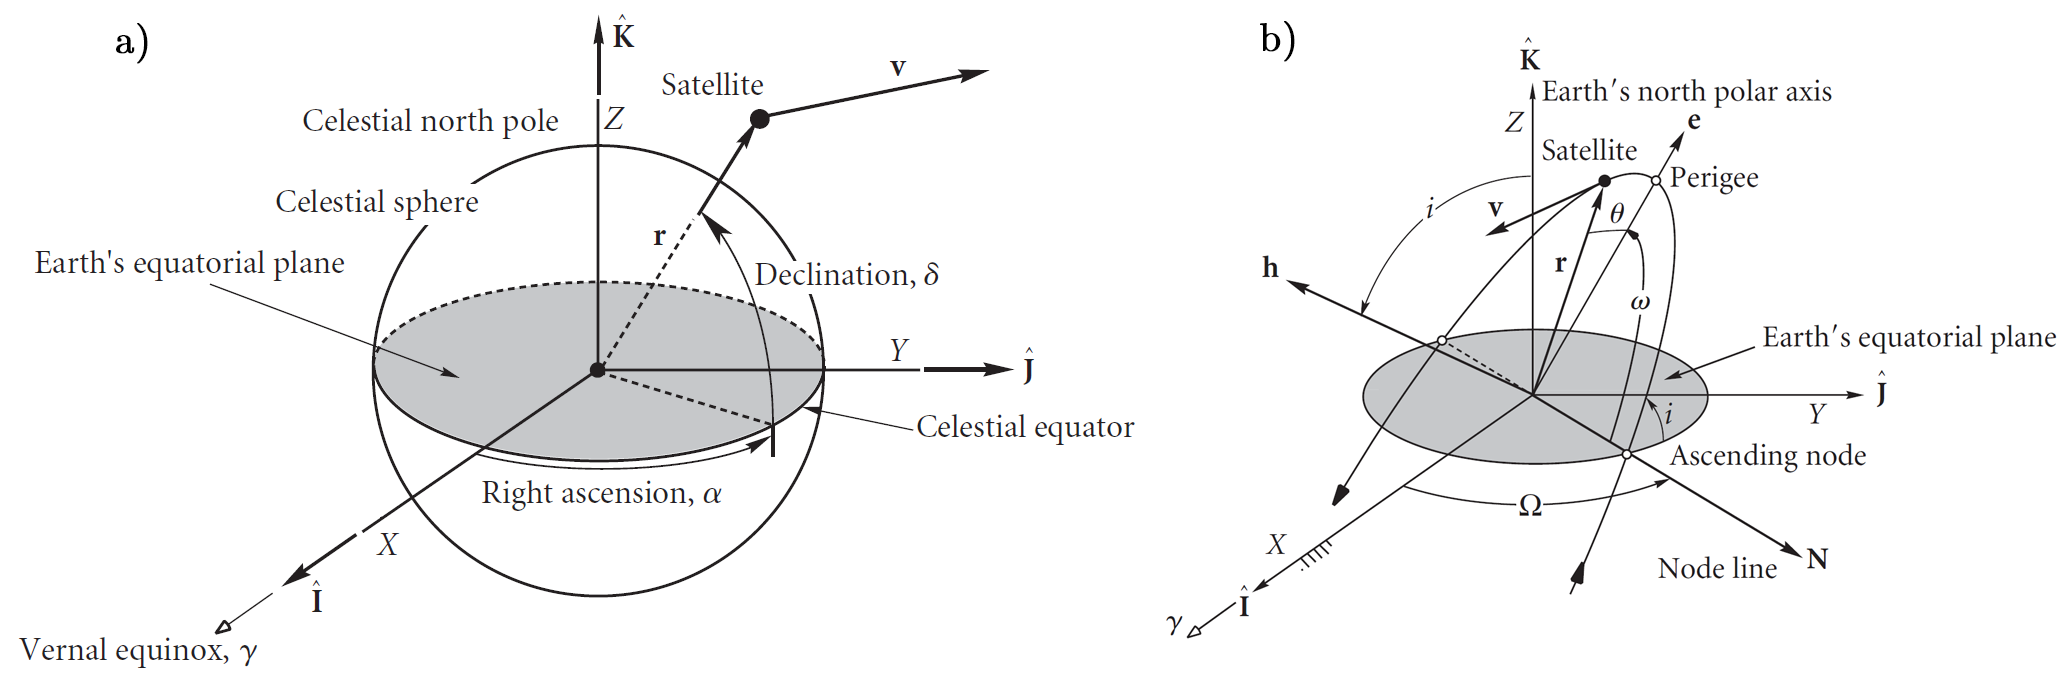
\includegraphics[scale=.28]{./Geometry/fig-Ch1-Geometry/COE&eqframe.png}
\caption[a) Geocentric-equatorial frame and b) Classical Orbital Elements]{a) Geocentric-equatorial frame and b) Classical Orbital Elements. Extracted from \cite{Howard}.}
\label{fig:eqframe}
\end{figure}

By defining this system, any point in the space can be depicted by its position vector $r$ and its movement can be studied by the velocity vector $\dot{r}$. These elements are useful especially for computational work, but they nearly do not provide information about the orbit. For these reason, the orbital elements were developed. More information on orbital elements in [\cite[Chapter 1, Section 1]{annex1}.